\chapter[Demonstração da Suíte de Testes Automatizados]{\textbf{\uppercase{Demonstração da Suíte de Testes Automatizados}}}
%\chapter[Resultados Alcançados]{\textbf{R}esultados \textbf{A}lcançados}
%\addcontentsline{toc}{chapter}{Resultados Alcançados}

\textit{Será apresentado neste capítulo a demostração da suíte de testes automatizados sob a solução abordada nas seções anteriores, e exposto os resultados que foram alcançados.}


\section{\textbf{\uppercase{Preparação do Ambiente de teste}}}

A demonstração da suíte de testes automatizados sobre a solução de integração dos sistemas, foram planejados em um ambiente controlado na elaboração e análise dos cenários de testes envolvidos. 

Para que os cenários de testes sejam o mais semelhante ao ambiente de produção, os mesmos foram executados sobre uma chamada telefônica tendo como originador da ligação um cliente com suas características especificadas e descritas em cada cenário de teste. 

O ambiente para execução dos testes ocorreu sobre um terminal cujo as especificações estão descritas abaixo:

\begin{table}[htb]
	\footnotesize
	\caption{Recursos computacionais utilizados}
	\label{tabela:recursosUtilizados}
	\begin{tabular}{|p{3.5cm}|p{3cm}|p{2cm}|p{4cm}|} \hline
		\textbf{SISTEMA OPER.} 	& \textbf{PROCESSADOR} 				& \textbf{MEMÓRIA} 	& \textbf{ARMAZENAMENTO}  \\ \hline
		Windows 7 64 bits 		& Intel Core i7-3520M CPU@2.9GHz 	& 8GB DDR3			& 1TB 5400 rpm \\ \hline
	\end{tabular}
	\legend{\fontsize{10}{12}\selectfont {Fonte: Autoria Própria}.}
\end{table}

Este terminal é responsável em executar ambos os sistemas envolvidos, no entanto como o software Asterisk está disponível somente para plataforma Linux, é preciso utilizar o recurso de máquina virtual através do software Virtual Box\footnote{Disponível em \url{https://www.virtualbox.org/}}, para executar uma instância da distribuição Disc-Os conforme citado nas seções anteriores.
 
O terminal possui uma conexão de rede local ativa, para que seja atribuído um endereço IP ao sistema operacional hospedeiro e ao convidado.

Visando garantir o correto funcionamento e a padronização do ambiente de teste foram criados testes de integração reproduzindo uma chamada telefônica programaticamente simulando um ambiente real, para tanto foi necessário utilizar os seguintes recursos o \textit{framework} JUnit na construção dos testes e o recurso nativo do Asterisk chamado \textit{Local Channel}.

Dessa forma é possível criar um canal de comunicação com um contexto e extensão específica dentro do sistema Asterisk, ou seja permite acessar diretamente o ponto de integração entre os sistemas.

Foram criados contextos específicos para teste no software Asterisk, replicando os mesmos contextos utilizados no fluxo da URA visando 
isolar o comportamento que ocorre no momento da integração sem a necessidade de redirecionamentos entre serviços ou ramais, conforme visto abaixo:

\begin{figure}[H]
	\centering
	\caption{Declaração dos contextos de teste no Asterisk}
	\label{figura:contextoTeste}
	\begin{subfigure}[H]{\textwidth}
		\centering
		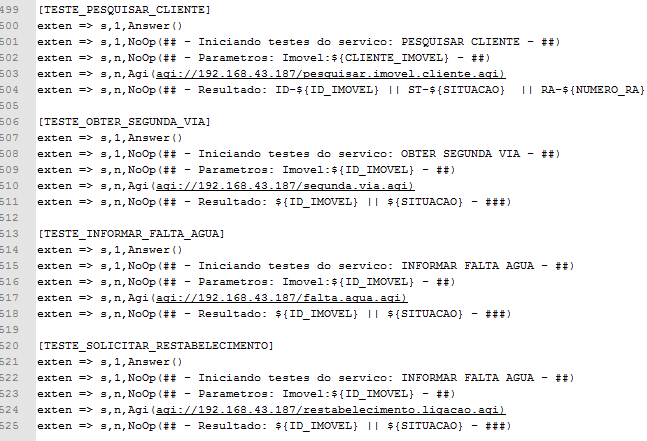
\includegraphics{figuras/contexto_teste.png}
		\legend {\fontsize{10}{12}\selectfont {Fonte: Autoria Própria}.}	
	\end{subfigure}
\end{figure}
	

\section{\textbf{\uppercase{Cenários de Teste}}}
Nesta fase foram elaborados possíveis cenários de teste para os três serviços automatizados, são respectivamente Obter 2ª via de conta, Informar Falta de Água e Solicitar Restabelecimento da Ligação de Água. Cada serviço proposto possui um objetivo específico sempre vinculado a um imóvel e/ou cliente.
Os cenários de testes representam as possíveis situações cadastrais fictícias e comportamentais vinculadas a um cliente, essencial para realizar um atendimento via sistema. Foram propostos 3 cenários de teste para cada serviço, visando assegurar o correto comportamento da solução. Abaixo estão descritos os cenários conforme cada serviço proposto:

\subsection{\textbf{\uppercase{Obter 2\textordfeminine \space Via de Conta}}}
Este serviço tem como objetivo checar se há alguma conta pendente referente ao imóvel informado, caso haja pendência o serviço deve submeter a conta pendente via e-mail para o cliente do imóvel. 

Abaixo são descritos os casos de testes previstos para o serviço obter 2ª Via de Conta, foi cadastrado o mesmo endereço de e-mail para os 3 cenários.
\begin{flushleft}
	\begin{description}
		\item \textbf{CENÁRIO 1}: Cliente devidamente cadastrado no Sistema, atualmente usuário de um imóvel que possui ativo a Ligação de Água e Esgoto, com uma conta em atraso. O Cliente deseja obter a conta em aberto, conforme demostrado na figura \ref{figura:2ViaCenario1}.
		
		\begin{figure}[H]
			\centering
			\caption{Obter 2ª via - Cenário de Teste 1}
			\label{figura:2ViaCenario1}
			\begin{subfigure}[H]{\textwidth}
				\centering
				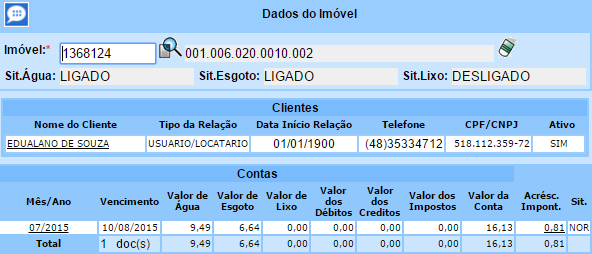
\includegraphics{figuras/cenarios/segunda_via/cenario_1.PNG}
				\legend {\fontsize{10}{12}\selectfont {Fonte: Autoria Própria}.}	
			\end{subfigure}
		\end{figure}
	\end{description}
	
	\begin{description}
		\item \textbf{CENÁRIO 2}: Cliente devidamente cadastrado no Sistema, atualmente sendo usuário de um imóvel que possui a Ligação de Água cortada por falta de pagamento, atualmente com três contas em aberto. O Cliente deseja obter a conta de maior atraso, conforme demostrado na figura \ref{figura:2ViaCenario2}.
		\begin{figure}[H]
			\centering
			\caption{Obter 2ª via - Cenário de Teste 2}
			\label{figura:2ViaCenario2}
			\begin{subfigure}[H]{\textwidth}
				\centering
				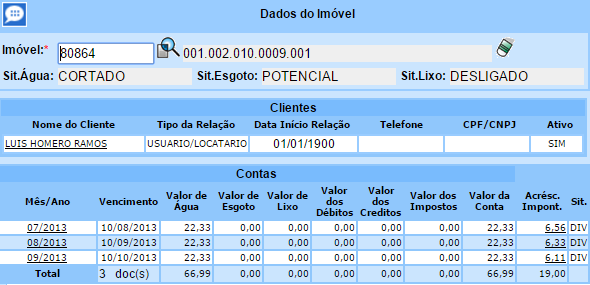
\includegraphics{figuras/cenarios/segunda_via/cenario_2.PNG}
				\legend {\fontsize{10}{12}\selectfont {Fonte: Autoria Própria}.}	
			\end{subfigure}
		\end{figure}
	\end{description}
	
	\begin{description}
		\item \textbf{CENÁRIO 3}: Cliente sem e-mail cadastrado no Sistema, atualmente sendo proprietário por dois imóveis que possuem ativo a Ligação de Água, possuindo várias contas pendentes para cada imóvel. O Cliente pretende obter todas as contas de todos os imóveis, conforme demostrado na figura \ref{figura:2ViaCenario3}.
		\begin{figure}[H]
			\centering
			\caption{Obter 2ª via - Cenário de Teste 3}
			\label{figura:2ViaCenario3}
			\begin{subfigure}[H]{\textwidth}
				\centering
				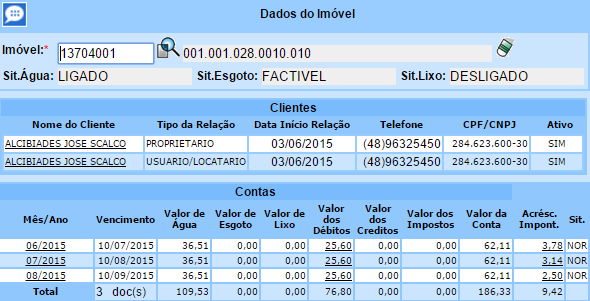
\includegraphics{figuras/cenarios/segunda_via/cenario_3.PNG}
				\legend {\fontsize{10}{12}\selectfont {Fonte: Autoria Própria}.}	
			\end{subfigure}
		\end{figure}
	\end{description}
	
\end{flushleft}


\subsection{\textbf{\uppercase{Informar Falta de Água}}}
Este serviço tem como objetivo formalizar junto ao sistema GSAN um novo Registro de Atendimento referente a Falta de Água para o imóvel informado.
Abaixo são descritos os casos de testes previstos para o serviço Informar Falta de Água.
\begin{flushleft}
	\begin{description}
		\item \textbf{CENÁRIO 1}: Cliente devidamente cadastrado no Sistema, atualmente locatário de um imóvel que possui ativo a Ligação de Água e Esgoto, com pendência de duas contas, com problemas no abastecimento de água. O Cliente pretende informar a falta de água para o imóvel, conforme demostrado na figura \ref{figura:informarFaltaAguaCenario1}.
		\begin{figure}[H]
			\centering
			\caption{Informar Falta de Água - Cenário de Teste 1}
			\label{figura:informarFaltaAguaCenario1}
			\begin{subfigure}[H]{\textwidth}
				\centering
				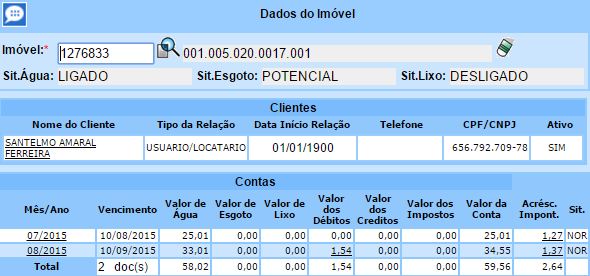
\includegraphics{figuras/cenarios/informar_falta_agua/cenario_1.PNG}
				\legend {\fontsize{10}{12}\selectfont {Fonte: Autoria Própria}.}	
			\end{subfigure}
		\end{figure}
	\end{description}
	
	\begin{description}
		\item \textbf{CENÁRIO 2}: Cliente sem e-mail cadastrado no Sistema, atualmente usuário de um único imóvel que possui ativo a Ligação de Água, com situação de adimplência, com problemas no abastecimento de água. O Cliente pretende informar a falta de água para o único imóvel, conforme demostrado na figura \ref{figura:informarFaltaAguaCenario1}.
		\begin{figure}[H]
			\centering
			\caption{Informar Falta de Água - Cenário de Teste 2}
			\label{figura:informarFaltaAguaCenario2}
			\begin{subfigure}[H]{\textwidth}
				\centering
				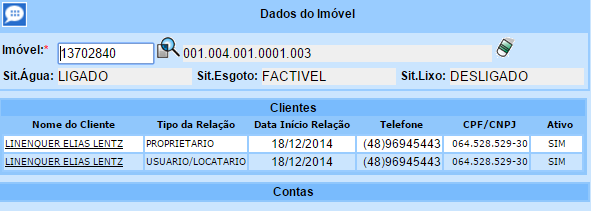
\includegraphics{figuras/cenarios/informar_falta_agua/cenario_2.PNG}
				\legend {\fontsize{10}{12}\selectfont {Fonte: Autoria Própria}.}	
			\end{subfigure}
		\end{figure}	
	\end{description}
	
	\begin{description}
		\item \textbf{CENÁRIO 3}: Cliente devidamente cadastrado no Sistema, atualmente proprietário de dois imóveis, que possuem a Ligação de Água ativa, em situação de inadimplência. O Cliente deseja informar problemas no abastecimento de água do imóvel específico onde reside, conforme demostrado na figura \ref{figura:informarFaltaAguaCenario3}.
		\begin{figure}[H]
			\centering
			\caption{Informar Falta de Água - Cenário de Teste 3}
			\label{figura:informarFaltaAguaCenario3}
			\begin{subfigure}[H]{\textwidth}
				\centering
				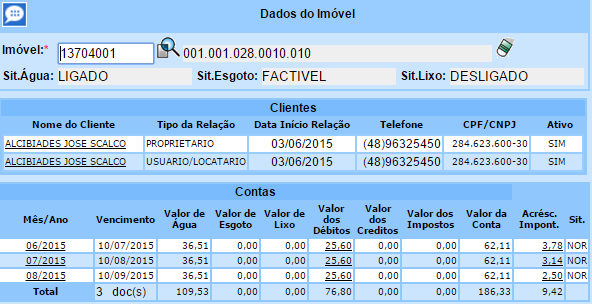
\includegraphics{figuras/cenarios/informar_falta_agua/cenario_3.PNG}
				\legend {\fontsize{10}{12}\selectfont {Fonte: Autoria Própria}.}	
			\end{subfigure}
		\end{figure}
	\end{description}
\end{flushleft}	

\subsection{\textbf{\uppercase{Solicitar Restabelecimento da Ligação de Água}}}
Este serviço tem como objetivo formalizar junto ao sistema GSAN um novo Registro de Atendimento referente ao Restabelecimento da Ligação de Água para um imóvel informado.
Abaixo são descritos os casos de testes previstos para o serviço Solicitar Restabelecimento da Ligação de Água.
\begin{flushleft}
	\begin{description}
		\item \textbf{CENÁRIO 1}: Cliente devidamente cadastrado no Sistema, atualmente proprietário de um único imóvel que possui a Ligação de Água interrompida por corte, em situação recente de adimplência. O Cliente deseja solicitar restabelecimento da ligação para o imóvel, conforme demostrado na figura \ref{figura:restabelecimentoLigacaoCenario1}.
		\begin{figure}[H]
			\centering
			\caption{Restabelecimento da Ligação de Água - Cenário de Teste 1}
			\label{figura:restabelecimentoLigacaoCenario1}
			\begin{subfigure}[H]{\textwidth}
				\centering
				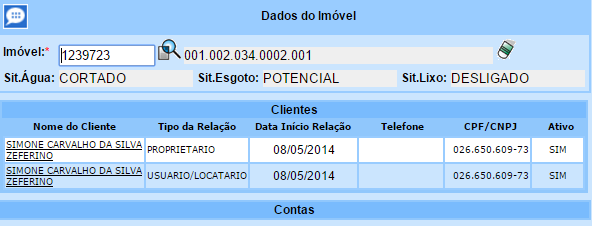
\includegraphics{figuras/cenarios/restabelecimento/cenario_1.PNG}
				\legend {\fontsize{10}{12}\selectfont {Fonte: Autoria Própria}.}	
			\end{subfigure}
		\end{figure}
	\end{description}
	
	\begin{description}
		\item \textbf{CENÁRIO 2}: Cliente devidamente cadastrado no Sistema, atualmente usuário de um único imóvel que possui a Ligação de Água interrompida por corte, em situação recente de adimplência. O Cliente deseja solicitar restabelecimento da ligação para o imóvel, conforme demostrado na figura \ref{figura:restabelecimentoLigacaoCenario2}.
		\begin{figure}[H]
			\centering
			\caption{Restabelecimento da Ligação de Água - Cenário de Teste 2}
			\label{figura:restabelecimentoLigacaoCenario2}
			\begin{subfigure}[H]{\textwidth}
				\centering
				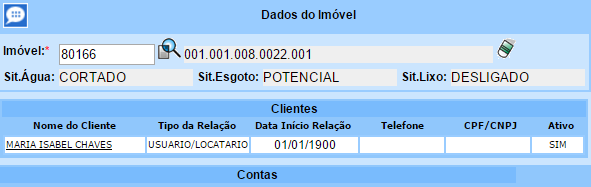
\includegraphics{figuras/cenarios/restabelecimento/cenario_2.PNG}
				\legend {\fontsize{10}{12}\selectfont {Fonte: Autoria Própria}.}	
			\end{subfigure}
		\end{figure}
	\end{description}
	
	\begin{description}
		\item \textbf{CENÁRIO 3}: Cliente devidamente cadastrado no Sistema, atualmente proprietário de um imóvel, que possui Ligação de Água interrompida por corte, devido a falta de pagamento das várias contas em aberto. O Cliente deseja solicitar restabelecimento da ligação para o imóvel sem realizar a negociação das faturas, conforme demostrado na figura \ref{figura:restabelecimentoLigacaoCenario3}.
		\begin{figure}[H]
			\centering
			\caption{Restabelecimento da Ligação de Água - Cenário de Teste 3}
			\label{figura:restabelecimentoLigacaoCenario3}
			\begin{subfigure}[H]{\textwidth}
				\centering
				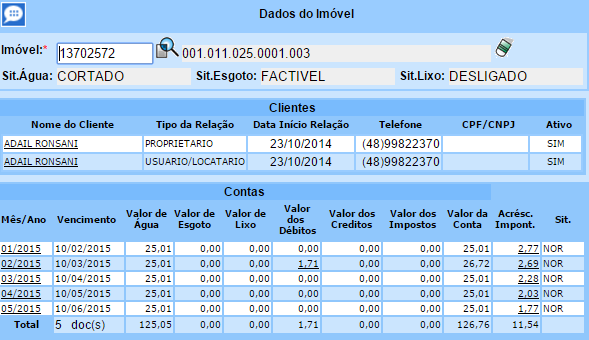
\includegraphics{figuras/cenarios/restabelecimento/cenario_3.PNG}
				\legend {\fontsize{10}{12}\selectfont {Fonte: Autoria Própria}.}	
			\end{subfigure}
		\end{figure}
	\end{description}

\end{flushleft}	


\section{\textbf{\uppercase{Execução dos Cenários de Teste}}}


A execução dos cenários propostos foi realizado utilizando o \textit{framework} de teste JUnit citados na seção anterior, segue abaixo resultado; 

\subsection{\textbf{\uppercase{Obter 2\textordfeminine  \space Via de Conta}}}
 
 Após a execução dos cenários de teste implementados para este serviço foi possível notar que 2/3 Cenários concluíram com sucesso e apenas 1/3 falhou em sua execução, a falha ocorreu no cenário 3 devido o cliente não possuir e-mail cadastrado no sistema, conforme demostrado na figura \ref{figura:segundaViaJUnit}.	
 \begin{figure}[H]
 	\centering
		\caption{Obter 2ª Via de Conta - Detalhes execução dos testes}
		\label{figura:segundaViaJUnit}
 	\begin{subfigure}[H]{\textwidth}
 		\centering
 		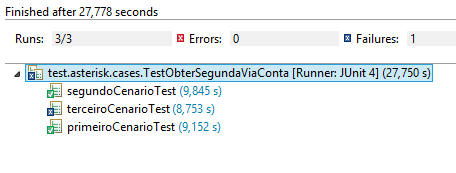
\includegraphics{figuras/cenarios/segunda_via/junit_result.PNG}
 		\legend {\fontsize{10}{12}\selectfont {Fonte: Autoria Própria}.}	
 	\end{subfigure}
 \end{figure}	
	

Em cada cenário de teste o sistema deve enviar um e-mail contendo a 2ª via da conta solicitada, a figura \ref{figura:emailRecebido} ilustra a caixa de entrada do E-mail configurado para cada cliente.
\begin{figure}[H]
	\centering
	\caption{Obter 2ª Via de Conta - E-mail recebido pelo cliente}
	\label{figura:emailRecebido}
	\begin{subfigure}[H]{\textwidth}
		\centering
		
\includegraphics{figuras/cenarios/segunda_via/envio_email.PNG}
		\legend {\fontsize{10}{12}\selectfont {Fonte: Autoria Própria}.}	
	\end{subfigure}
\end{figure}

	
\subsection{\textbf{\uppercase{Informar Falta de Água}}}

 Após a execução dos cenários de teste implementados para este serviço foi possível identificar que todos os 3 cenários previstos executaram com sucesso, conforme demostrado na figura \ref{figura:informarFaltaJUnit}.	

	\begin{figure}[H]
		\centering
		\caption{Informar Falta de Água - Detalhes execução dos testes}
		\label{figura:informarFaltaJUnit}
		\begin{subfigure}[H]{\textwidth}
			\centering
			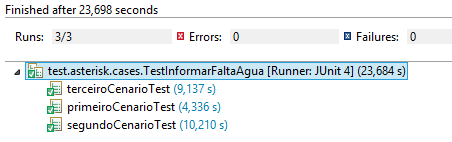
\includegraphics{figuras/cenarios/informar_falta_agua/junit_result.PNG}
			\legend {\fontsize{10}{12}\selectfont {Fonte: Autoria Própria}.}	
		\end{subfigure}
	\end{figure}

Ao consulta o sistema GSAN, visando identificar se houve a ocorrência da formalização dos Registros de Atendimentos, o primeiro cenário cujo o identificador 1276833 representa a matrícula do imóvel, houve a geração do Registro de Atendimento de número 6594, conforme demonstrado na figura \ref{figura:informarFaltaRA1}.

\begin{figure}[H]
	\centering
		\caption{Informar Falta de Água - RA gerado para o Cenário 1}
		\label{figura:informarFaltaRA1}
	\begin{subfigure}[H]{\textwidth}
		\centering
		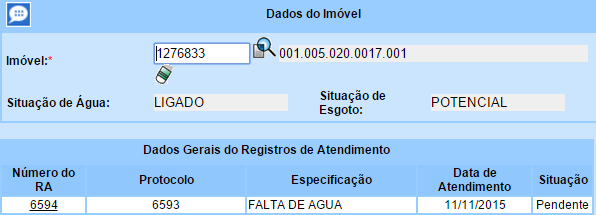
\includegraphics{figuras/cenarios/informar_falta_agua/resultado_1.PNG}
		\legend {\fontsize{10}{12}\selectfont {Fonte: Autoria Própria}.}	
	\end{subfigure}
\end{figure}

	
Para o segundo cenário, cujo o identificador 13702840 representa a matrícula do imóvel, houve a geração do Registro de Atendimento de número 6598, conforme exposto na figura \ref{figura:informarFaltaRA2}.	
		
\begin{figure}[H]
	\centering
	\caption{Informar Falta de Água - RA gerado para o Cenário 2}
	\label{figura:informarFaltaRA2}
	\begin{subfigure}[H]{\textwidth}
		\centering
		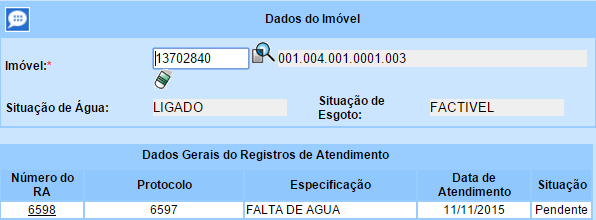
\includegraphics{figuras/cenarios/informar_falta_agua/resultado_2.PNG}
		\legend {\fontsize{10}{12}\selectfont {Fonte: Autoria Própria}.}	
	\end{subfigure}
\end{figure}

Para o terceiro cenário, cujo o identificador 13704001 representa a matrícula do imóvel, também houve a geração do Registro de Atendimento de número 6596, conforme exposto na figura \ref{figura:informarFaltaRA3}.	

\begin{figure}[H]
	\centering
	\caption{Informar Falta de Água - RA gerado para o Cenário 3}
	\label{figura:informarFaltaRA3}
	\begin{subfigure}[H]{\textwidth}
		\centering
		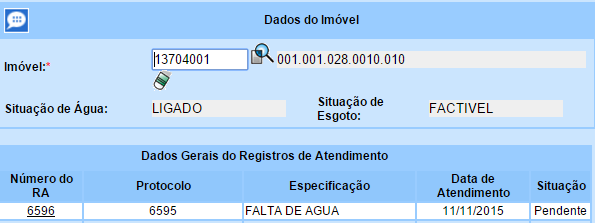
\includegraphics{figuras/cenarios/informar_falta_agua/resultado_3.PNG}
		\legend {\fontsize{10}{12}\selectfont {Fonte: Autoria Própria}.}	
	\end{subfigure}
\end{figure}

		
\subsection{\textbf{\uppercase{Solicitar Restabelecimento da Ligação de Água}}}

 Após a execução dos cenários de teste implementados para este serviço foi possível identificar que todos os 3 cenários previsto executaram com sucesso, conforme demostrado na figura \ref{figura:restabelecimentoJUnit}.	

\begin{figure}[H]
	\centering
	\caption{Restabelecimento da Ligação de Água - Detalhes execução dos testes}
	\label{figura:restabelecimentoJUnit}
	\begin{subfigure}[H]{\textwidth}
		\centering
		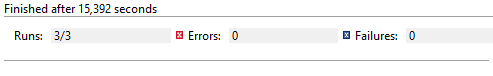
\includegraphics{figuras/cenarios/restabelecimento/junit_result.PNG}
		\legend {\fontsize{10}{12}\selectfont {Fonte: Autoria Própria}.}	
	\end{subfigure}
\end{figure}

Ao consulta o sistema GSAN, visando identificar se houve a ocorrência da formalização dos Registros de Atendimentos, o primeiro cenário cujo o identificar 1239723 representa a matrícula do imóvel, houve a geração do Registro de Atendimento de número 6604, conforme demonstrado na figura \ref{figura:restabelecimentoRA1}.

\begin{figure}[H]
	\centering
	\caption{Restabelecimento da Ligação de Água - RA gerado para o Cenário 1}
	\label{figura:restabelecimentoRA1}
	\begin{subfigure}[H]{\textwidth}
		\centering
		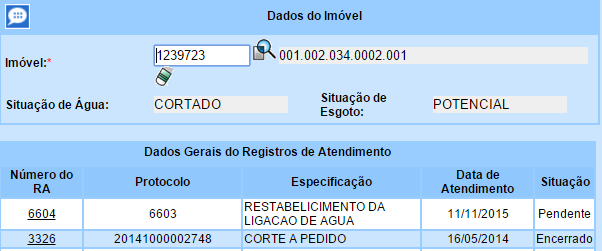
\includegraphics{figuras/cenarios/restabelecimento/resultado_1.PNG}
		\legend {\fontsize{10}{12}\selectfont {Fonte: Autoria Própria}.}	
	\end{subfigure}
\end{figure}


Para o segundo cenário, cujo o identificador 80166 representa a matrícula do imóvel, houve a geração do Registro de Atendimento de número 6608, conforme exposto na figura \ref{figura:restabelecimentoRA2}.	

\begin{figure}[H]
	\centering
	\caption{Restabelecimento da Ligação de Água - RA gerado para o Cenário 2}
	\label{figura:restabelecimentoRA2}
	\begin{subfigure}[H]{\textwidth}
		\centering
		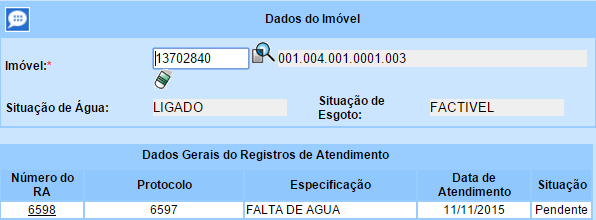
\includegraphics{figuras/cenarios/informar_falta_agua/resultado_2.PNG}
		\legend {\fontsize{10}{12}\selectfont {Fonte: Autoria Própria}.}	
	\end{subfigure}
\end{figure}

	
Para o terceiro cenário, cujo o identificador 13702572 representa a matrícula do imóvel, mesmo o cliente em situação de inadimplência houve a geração do Registro de Atendimento de número 6606, conforme exposto na figura \ref{figura:restabelecimentoRA3}.	

\begin{figure}[H]
	\centering
	\caption{Restabelecimento da Ligação de Água - RA gerado para o Cenário 3}
	\label{figura:restabelecimentoRA3}
	\begin{subfigure}[H]{\textwidth}
		\centering
		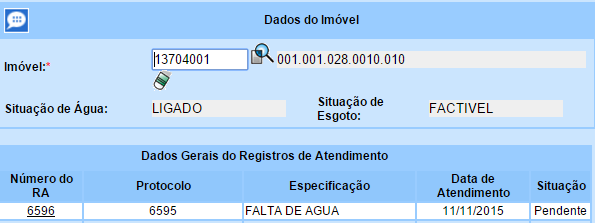
\includegraphics{figuras/cenarios/informar_falta_agua/resultado_3.PNG}
		\legend {\fontsize{10}{12}\selectfont {Fonte: Autoria Própria}.}	
	\end{subfigure}
\end{figure}


Nos testes houve somente 1 falha conforme esperado no teste do Serviço Obter 2ª via de conta, onde o cliente não havia o e-mail cadastral, já nos outros testes a solução se comportou de forma estável pois todas as solicitações para Informar Falta de Água e Solicitar Restabelecimento da Ligação de Água foram atendidas e formalizadas junto ao sistema GSAN de forma automatizada.

Os detalhes sobre cada Registro de Atendimento mencionado acima podem ser consultados nas apêndices deste trabalho.
